\documentclass[a4paper]{article}
\usepackage[fontset=fandol]{ctex}
\usepackage[margin=2cm]{geometry}
\usepackage{pdfpages}
\usepackage{hyperref}
\usepackage{longtable}
\title{Stanford CS231N: Deep Learning for Computer Vision (Spring 2025)}
\author{Codex based on course page, slides, subtitles, and lecture videos}
\date{\today}
\begin{document}
\maketitle
\tableofcontents
\newpage
\section*{课程说明}
本讲义先逐讲生成，再按播放列表顺序合并。
\addcontentsline{toc}{section}{课程说明}
\section*{课程目录}
\addcontentsline{toc}{section}{课程目录}
\begin{longtable}{p{0.08\textwidth}p{0.67\textwidth}p{0.18\textwidth}}
\textbf{讲次} & \textbf{主题} & \textbf{日期}\\
\hline
01 & Lecture 1: Introduction & 2025-04-01\\
02 & Lecture 2: Image Classification with Linear Classifiers & 2025-04-03\\
03 & Lecture 3: Regularization and Optimization & 2025-04-08\\
04 & Lecture 4: Neural Networks and Backpropagation & 2025-04-10\\
05 & Lecture 5: Image Classification with CNNs & 2025-04-15\\
06 & Lecture 6: CNN Architectures & 2025-04-17\\
07 & Lecture 7: Recurrent Neural Networks & 2025-04-22\\
08 & Lecture 8: Attention and Transformers & 2025-04-24\\
09 & Lecture 9: Object Detection, Image Segmentation, Visualizing and Understanding & 2025-04-29\\
10 & Lecture 10: Video Understanding & 2025-05-01\\
11 & Lecture 11: Large Scale Distributed Training & 2025-05-06\\
12 & Lecture 12: Self-supervised Learning & 2025-05-08\\
13 & Lecture 13:  Generative Models 1 & 2025-05-15\\
14 & Lecture 14:  Generative Models 2 & 2025-05-20\\
15 & Lecture 15: 3D Vision & 2025-05-22\\
16 & Lecture 16: Vision and Language & 2025-05-27\\
17 & Lecture 17: Robot Learning & 2025-05-29\\
18 & Lecture 18: Human-Centered AI & 2025-06-03\\
\end{longtable}

\section{Lecture 1: Introduction}

\includepdf[pages=-,pagecommand={\thispagestyle{plain}}]{../lectures/01_introduction/lecture_01_note.pdf}

\section{Lecture 2: Image Classification with Linear Classifiers}

\includepdf[pages=-,pagecommand={\thispagestyle{plain}}]{../lectures/02_image_classification_with_linear_classifiers/lecture_02_note.pdf}

\section{Lecture 3: Regularization and Optimization}

\includepdf[pages=-,pagecommand={\thispagestyle{plain}}]{../lectures/03_regularization_and_optimization/lecture_03_note.pdf}

\section{Lecture 4: Neural Networks and Backpropagation}

\includepdf[pages=-,pagecommand={\thispagestyle{plain}}]{../lectures/04_neural_networks_and_backpropagation/lecture_04_note.pdf}

\section{Lecture 5: Image Classification with CNNs}

\includepdf[pages=-,pagecommand={\thispagestyle{plain}}]{../lectures/05_image_classification_with_cnns/lecture_05_note.pdf}

\section{Lecture 6: CNN Architectures}

\includepdf[pages=-,pagecommand={\thispagestyle{plain}}]{../lectures/06_cnn_architectures/lecture_06_note.pdf}

\section{Lecture 7: Recurrent Neural Networks}

\includepdf[pages=-,pagecommand={\thispagestyle{plain}}]{../lectures/07_recurrent_neural_networks/lecture_07_note.pdf}

\section{Lecture 8: Attention and Transformers}

\includepdf[pages=-,pagecommand={\thispagestyle{plain}}]{../lectures/08_attention_and_transformers/lecture_08_note.pdf}

\section{Lecture 9: Object Detection, Image Segmentation, Visualizing and Understanding}

\includepdf[pages=-,pagecommand={\thispagestyle{plain}}]{../lectures/09_object_detection_image_segmentation_visualizing_and_understanding/lecture_09_note.pdf}

\section{Lecture 10: Video Understanding}

\includepdf[pages=-,pagecommand={\thispagestyle{plain}}]{../lectures/10_video_understanding/lecture_10_note.pdf}

\section{Lecture 11: Large Scale Distributed Training}

\includepdf[pages=-,pagecommand={\thispagestyle{plain}}]{../lectures/11_large_scale_distributed_training/lecture_11_note.pdf}

\section{Lecture 12: Self-supervised Learning}

\includepdf[pages=-,pagecommand={\thispagestyle{plain}}]{../lectures/12_self_supervised_learning/lecture_12_note.pdf}

\section{Lecture 13:  Generative Models 1}

\includepdf[pages=-,pagecommand={\thispagestyle{plain}}]{../lectures/13_generative_models_1/lecture_13_note.pdf}

\section{Lecture 14:  Generative Models 2}

\includepdf[pages=-,pagecommand={\thispagestyle{plain}}]{../lectures/14_generative_models_2/lecture_14_note.pdf}

\section{Lecture 15: 3D Vision}

\includepdf[pages=-,pagecommand={\thispagestyle{plain}}]{../lectures/15_3d_vision/lecture_15_note.pdf}

\section{Lecture 16: Vision and Language}

\includepdf[pages=-,pagecommand={\thispagestyle{plain}}]{../lectures/16_vision_and_language/lecture_16_note.pdf}

\section{Lecture 17: Robot Learning}
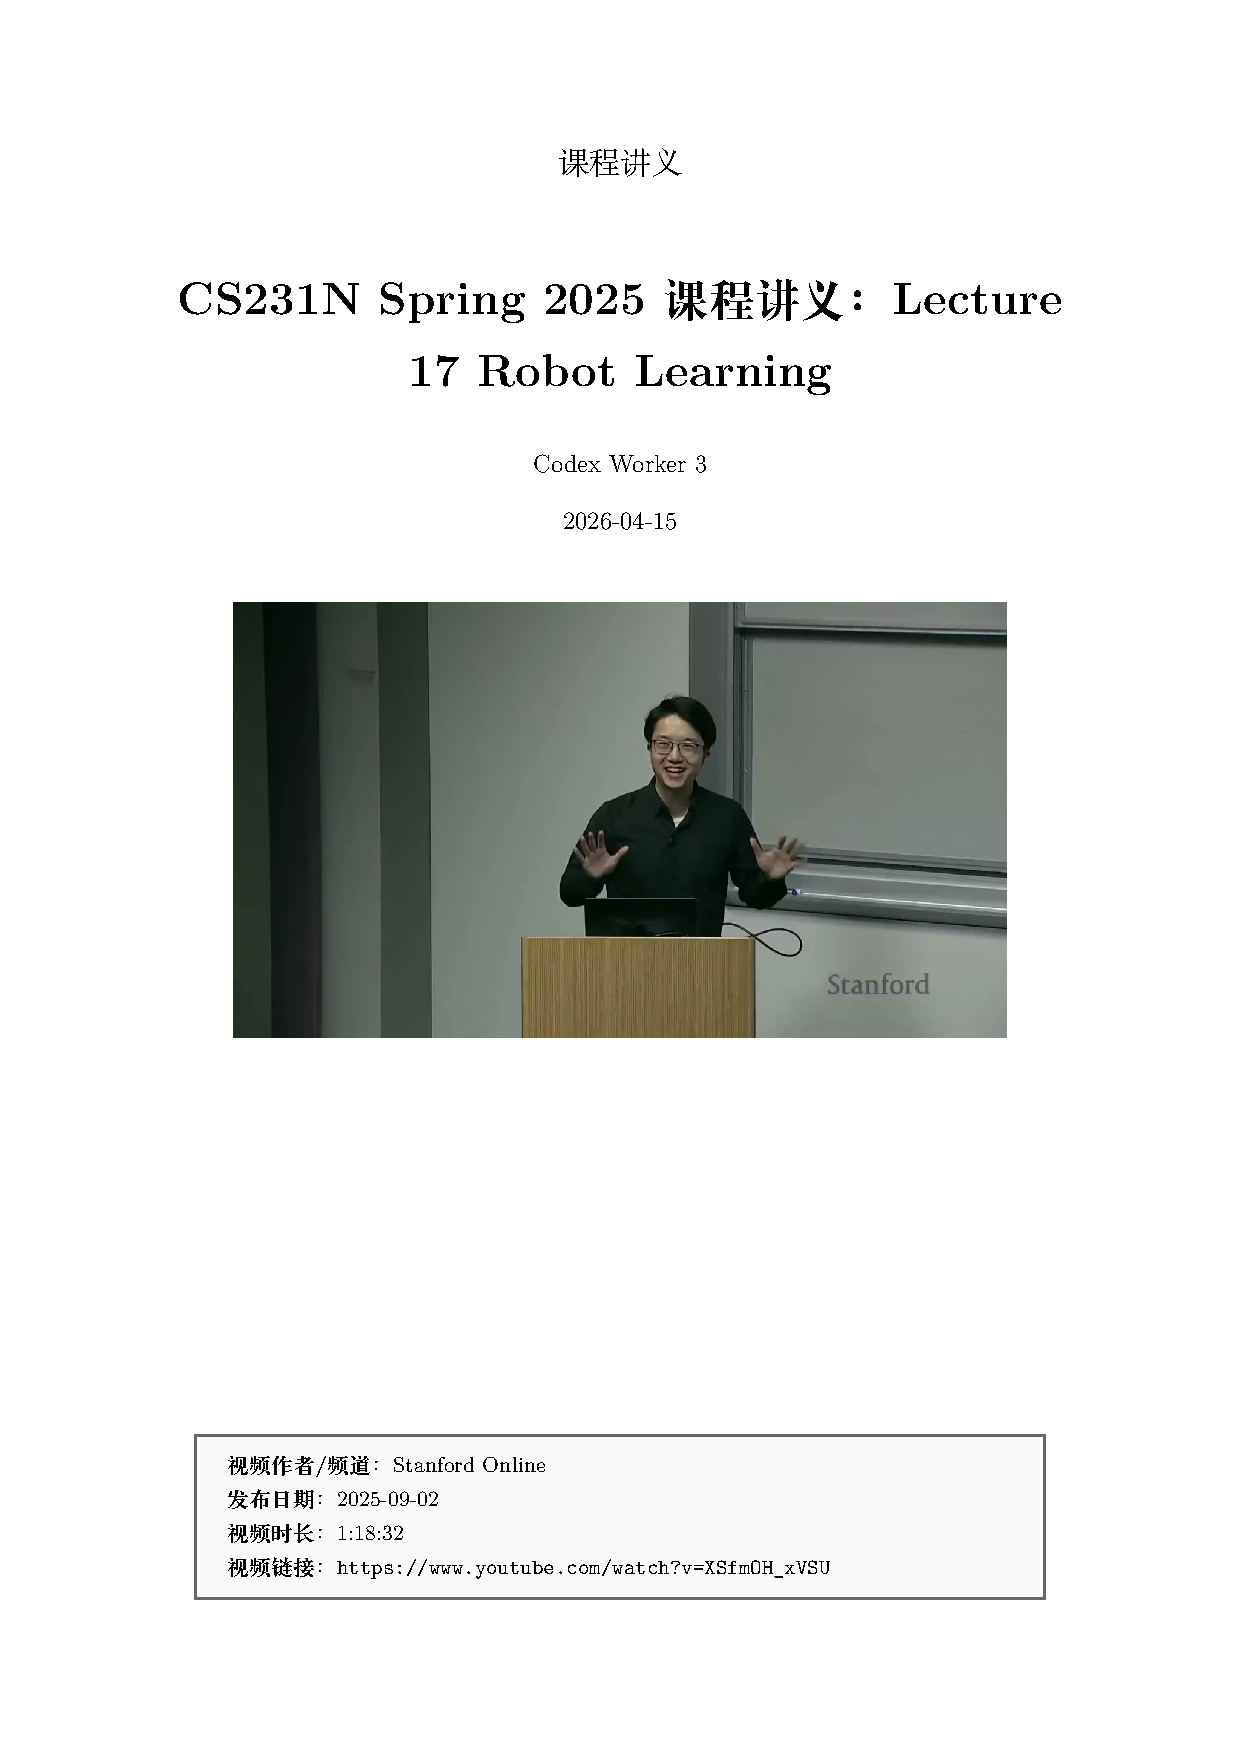
\includepdf[pages=-,pagecommand={\thispagestyle{plain}}]{../lectures/17_robot_learning/lecture_17_note.pdf}

\section{Lecture 18: Human-Centered AI}

\includepdf[pages=-,pagecommand={\thispagestyle{plain}}]{../lectures/18_human_centered_ai/lecture_18_note.pdf}

\end{document}
